\section{Desarrollo del \textit{frontend}}
\label{dev:sec:desarrollo_frontend}

Definida la base de datos y desarrollado el \textit{backend}, el \textit{frontend} es la última parte de la plataforma que resta por ser definido y desarrollado. El \textit{frontend} es la parte de la plataforma con la que el usuario interactúa directamente, y es la responsable de mostrar la información al usuario para que este pueda realizar las acciones que desee.

Existen mútliples tecnologías que permiten desarrollar el \textit{frontend} de una plataforma web, y en este caso se ha optado por utilizar React, un \textit{framework} de JavaScript que hoy en día es uno de los más utilizados para el desarrollo de aplicaciones web. Precisamente del hecho de que React sea un estándar de facto en el desarrollo de aplicaciones web, se deriva la decisión de haber utilizado esta tecnología. Es un \textit{framework} muy potente, respaldado por una gran cantidad de documentación y recursos, además de una enorme empresa como es Meta (anteriormente conocida como Facebook) que lo respalda y mantiene. Esto asegura que React se mantenga actualizado y sea compatible con las últimas tecnologías web.

A pesar de que React funciona con JavaScript, siguiendo lo mencionado en la sección \ref{mt:subsec:frontend}, se ha optado por utilizar TypeScript. TypeScript es un superconjunto de JavaScript que añade tipado estático y otras características que facilitan el desarrollo y mantenimiento del código. Esto permite detectar errores en tiempo de compilación, lo que mejora la calidad del código y reduce la probabilidad de errores en tiempo de ejecución. Estos aspectos son especialmente importantes en un proyecto de gran envergadura, donde la complejidad del código puede aumentar rápidamente. Como se pretende que la plataforma siga evolucionando y creciendo, el uso de TypeScript facilita la escalabilidad del proyecto y evita problemas a largo plazo.

Con estos puntos claros, se ha procedido a desarrollar el \textit{frontend} de la plataforma. Este proceso se ha dividido en principalmente dos fases: la estructuración del proyecto y el desarrollo de las diferentes vistas y componentes que componen la plataforma.

\subsection{Estructuración del proyecto}
\label{dev:subsec:estructuracion_proyecto}

Las estructuras de los proyectos desarrollados con React pueden variar dependiendo de las necesidades del proyecto y de las preferencias del equipo de desarrollo. Sin embargo, existen algunas convenciones y buenas prácticas que se suelen seguir para mantener el código organizado y fácil de mantener.

En este caso, se ha optado por una estructura que se divide en principalmente cuatro carpetas principales:

\begin{itemize}
    \item \texttt{src/components}: Esta carpeta reúne todos los componentes reutilizables de la aplicación. En React, los componentes son las unidades básicas que conforman la interfaz: pueden ir desde elementos sencillos como botones hasta estructuras más complejas como formularios completos. Para mantener una buena organización, se divide esta carpeta en subcarpetas: una para los componentes comunes (usados en múltiples partes de la aplicación) y otras para los componentes específicos de cada funcionalidad o sección.
    \item \texttt{src/routes}: En esta carpeta se encuentran definidas todas las rutas de la aplicación utilizando la librería @tanstack/react-router. La estructura de rutas sigue una organización jerárquica que refleja la navegación de la aplicación, permitiendo agrupar rutas relacionadas en subcarpetas. Cada archivo de ruta incluye tanto la definición del componente que debe renderizarse como los datos que necesita cargar.
    \item \texttt{src/services}: Esta carpeta contiene los servicios encargados de realizar las peticiones HTTP al \textit{backend} utilizando la librería axios. Cada servicio agrupa las funciones relacionadas con un recurso concreto de la aplicación (por ejemplo, pedidos o productos), lo que permite centralizar la lógica de comunicación con el servidor.
    \item \texttt{src/types}: Esta carpeta contiene tanto las definiciones de tipos TypeScript como los esquemas de validación de la aplicación. Los tipos se utilizan para garantizar una correcta tipificación del código en toda la aplicación, mejorando la seguridad y legibilidad. Por su parte, los esquemas, definidos con la librería zod, se emplean para validar los datos introducidos por el usuario antes de enviarlos al servidor, asegurando que cumplan con las reglas establecidas (por ejemplo, formatos, campos obligatorios o rangos de valores).
\end{itemize}

Esta estructura queda plasmada en la figura \ref{fig:dev:estructura_archivos}, donde se puede observar como se organizan las diferentes carpetas del proyecto. En la siguiente sección se detallará el desarrollo de las vistas y los componentes que componen cada una de ellas, lo que permitirá una mejor comprensión de la figura.

\begin{figure}
    \centering
    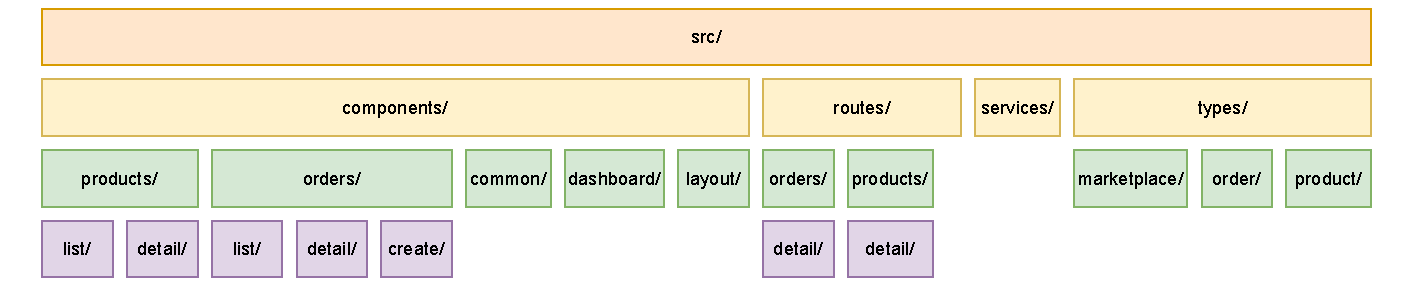
\includegraphics[width=0.95\textwidth]{figures/design_develop/estructura_archivos.pdf}
    \caption{Estructura de archivos del \textit{frontend} de la plataforma.}
    \label{fig:dev:estructura_archivos}
\end{figure}

\subsection{Desarrollo de vistas y componentes}
\label{dev:subsec:desarrollo_vistas_componentes}

Antes de comenzar con el desarrollo de las vistas, es fundamental tener claro cómo deben ser accesibles las distintas funcionalidades de la plataforma para el usuario final. Por este motivo, resulta útil remitir a la sección \ref{dev:subsec:bloques_funcionalidades}, donde se definieron los bloques funcionales principales. A modo de resumen, las funcionalidades clave que debe ofrecer la plataforma son las siguientes:

\begin{itemize}
    \item \textbf{Gestión de pedidos}:
          \begin{itemize}
              \item Centralización de los pedidos procedentes de los distintos canales de venta.
              \item Creación manual de nuevos pedidos.
              \item Edición de pedidos existentes.
          \end{itemize}
    \item \textbf{Gestión de productos}:
          \begin{itemize}
              \item Centralización de los productos provenientes de los distintos canales de venta.
              \item Asignación de productos a canales de venta específicos.
              \item Edición de productos ya existentes.
          \end{itemize}
\end{itemize}

El desarrollo de estas funcionalidades debe enfocarse en ofrecer una experiencia de usuario ágil e intuitiva, permitiendo una gestión eficiente de los canales de venta. El objetivo es que la plataforma se convierta en una herramienta imprescindible para la administración diaria de los distintos canales de venta.

Es importante señalar que los usuarios de la plataforma no disponen de permisos para crear ni editar canales de venta. La incorporación de un nuevo canal es una tarea gestionada exclusivamente por la plataforma, ya que implica un análisis previo, así como la implementación y configuración de la API correspondiente, entre otros aspectos técnicos. El usuario final puede asignar productos a los canales ya disponibles, pero no tiene control sobre su creación o configuración.

Anotado este último punto, se puede continuar con el desarrollo de las vistas. Teniendo en cuenta las funcionalidades definidas, la plataforma debe contar con dos vistas principales: una para la gestión de pedidos y otra para la gestión de productos. Como añadido a estas vistas, se ha incluido una vista de inicio que proporciona una visión general de la plataforma y permite observar datos generales del estado de los pedidos y productos.

Así pues, para centralizar las tres vistas principales se ha creado un menú lateral de navegación que permite al usuario acceder fácilmente a cada una de ellas, tal como se muestra en la figura \ref{fig:dev:ss:menu_lateral}. Este menú está presente en todas las vistas de la plataforma, permitiendo que el usuario pueda acceder a cada una de las secciones principales de forma rápida. De momento el menú cuenta con tres secciones: \textit{Dashboard}, \textit{Orders} y \textit{Products}. Sin embargo, está diseñado para que, en el futuro, se puedan añadir nuevas secciones fácilmente así permitiendo la expansión de nuevas funcionalidades.

\begin{figure}
    \centering
    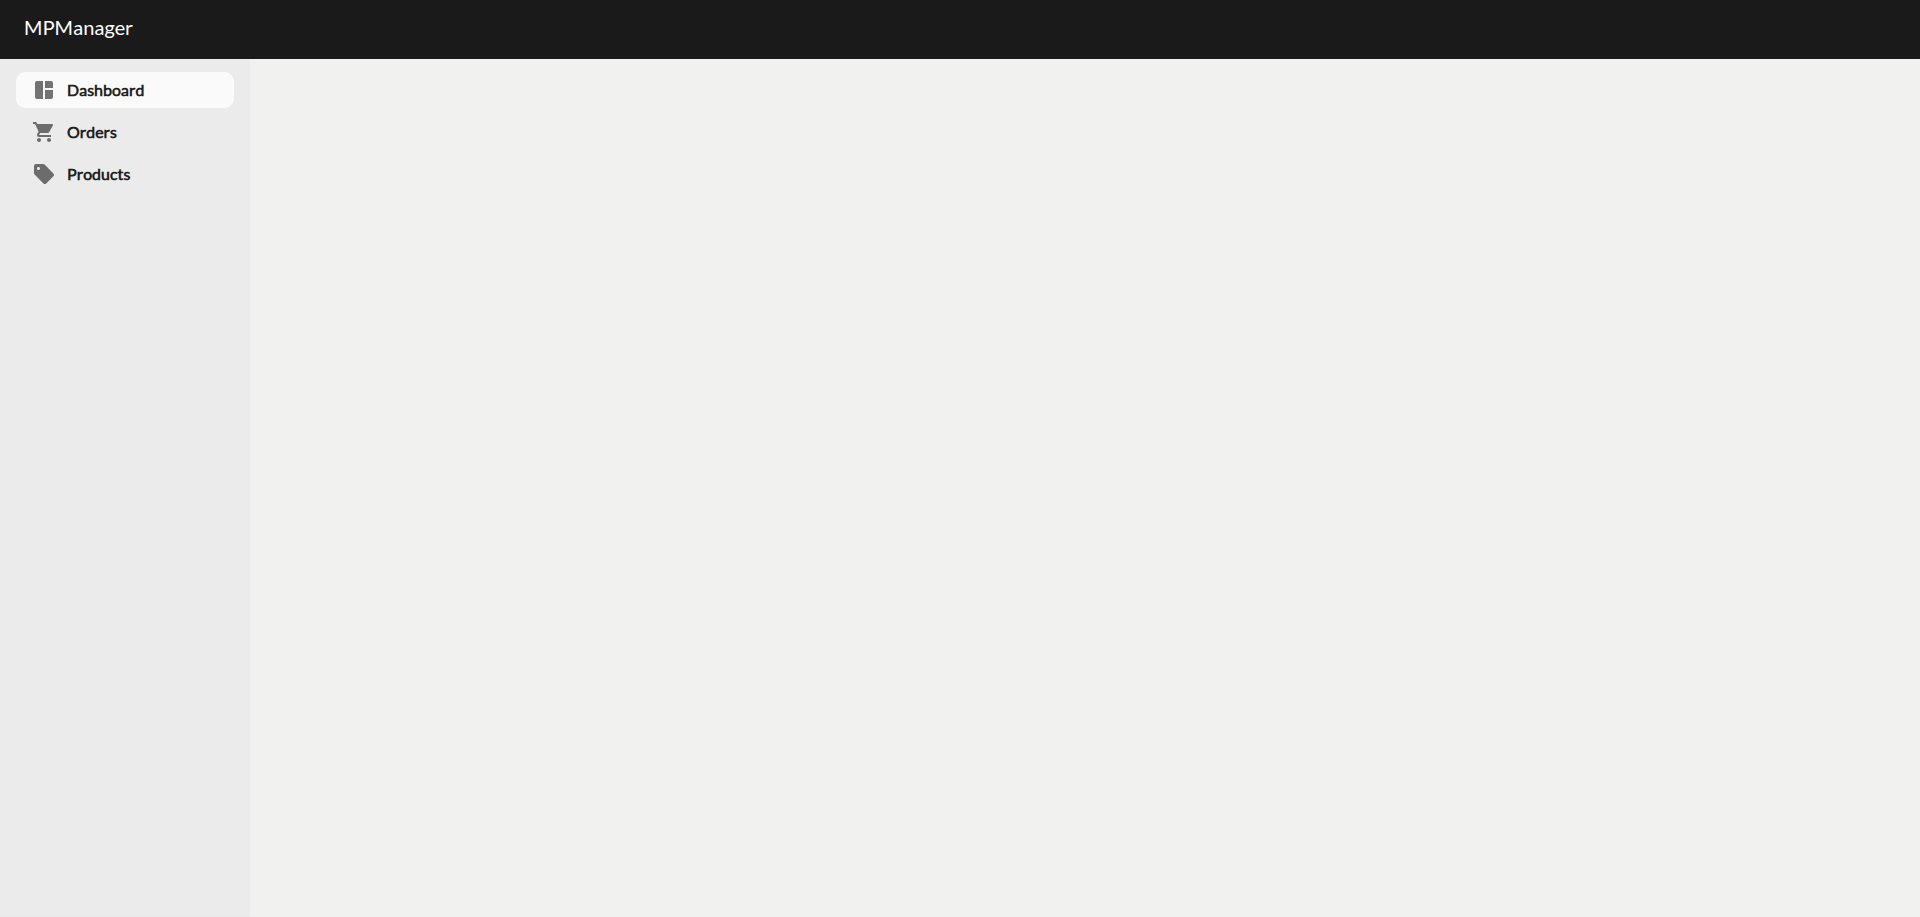
\includegraphics[width=0.8\textwidth]{figures/design_develop/screenshots/menu_lateral.png}
    \caption{Menú lateral de navegación de la plataforma.}
    \label{fig:dev:ss:menu_lateral}
\end{figure}

El orden de las secciones del menú lateral sigue una lógica que facilita la navegación. En primer lugar, se encuentra la sección \textit{Dashboard}, que proporciona una visión general del estado de la plataforma, permitiendo al usuario obtener información rápida sobre los pedidos y productos. A continuación, se sitúa la sección \textit{Orders}, que permite gestionar los pedidos de forma centralizada, y finalmente, la sección \textit{Products}, donde se pueden gestionar los productos disponibles en los distintos canales de venta. No obstante, el orden de desarrollo de las vistas no ha seguido este mismo orden, sino que se ha desarrollado primero la vista de pedidos, seguida de la vista de productos y, por último, la vista de inicio. El orden entre las vistas de pedidos y productos no es relevante, ya que ambas son bastante independientes una de la otra. Sin embargo, la vista de inicio se ha desarrollado al final para poder incluir en ella información relevante sobre el estado de los pedidos y productos, que se obtiene de las vistas anteriores. Por este mismo motivo, a continuación se detallará el desarrollo de las vistas según el orden con el que se han implementado, pues es seguramente el orden más lógico para comprender como todo funciona e interactúa.

\subsubsection{Vista de pedidos}
\label{dev:subsubsec:vista_pedidos}

La vista de pedidos es una de las más importantes de la plataforma, ya que permite gestionar todos los pedidos provenientes de los distintos canales de venta. Gestionar los pedidos implica poder verlos, editarlos y crear de nuevos. Así pues, dicha vista se ha dividido en dostres:

\begin{itemize}
    \item \textbf{Vista general de pedidos}: Esta vista permite al usuario ver todos los pedidos que ha recibido la plataforma, independientemente del canal de venta del que provengan. En esta vista se pueden filtrar los pedidos por el canal de ventas además de poder buscarlos por su identificador o el nombre del cliente.
    \item \textbf{Vista detallada de pedido}: Esta vista permite al usuario ver un pedido concreto, así como editarlo. En esta vista se pueden ver todos los detalles del pedido, incluyendo los productos que lo componen, el estado del pedido y la información del cliente. Además, se pueden realizar acciones como editar el estado del pedido o añadir nuevos productos al mismo.
    \item \textbf{Vista de creación de pedido}: Esta vista permite al usuario crear un nuevo pedido. En esta vista se pueden seleccionar los productos que componen el pedido, así como introducir la información del cliente y el canal de venta al que pertenece el pedido. Una vez creado el pedido, este se añadirá a la lista de pedidos y estará disponible para su gestión.
\end{itemize}

\begin{figure}
    \centering
    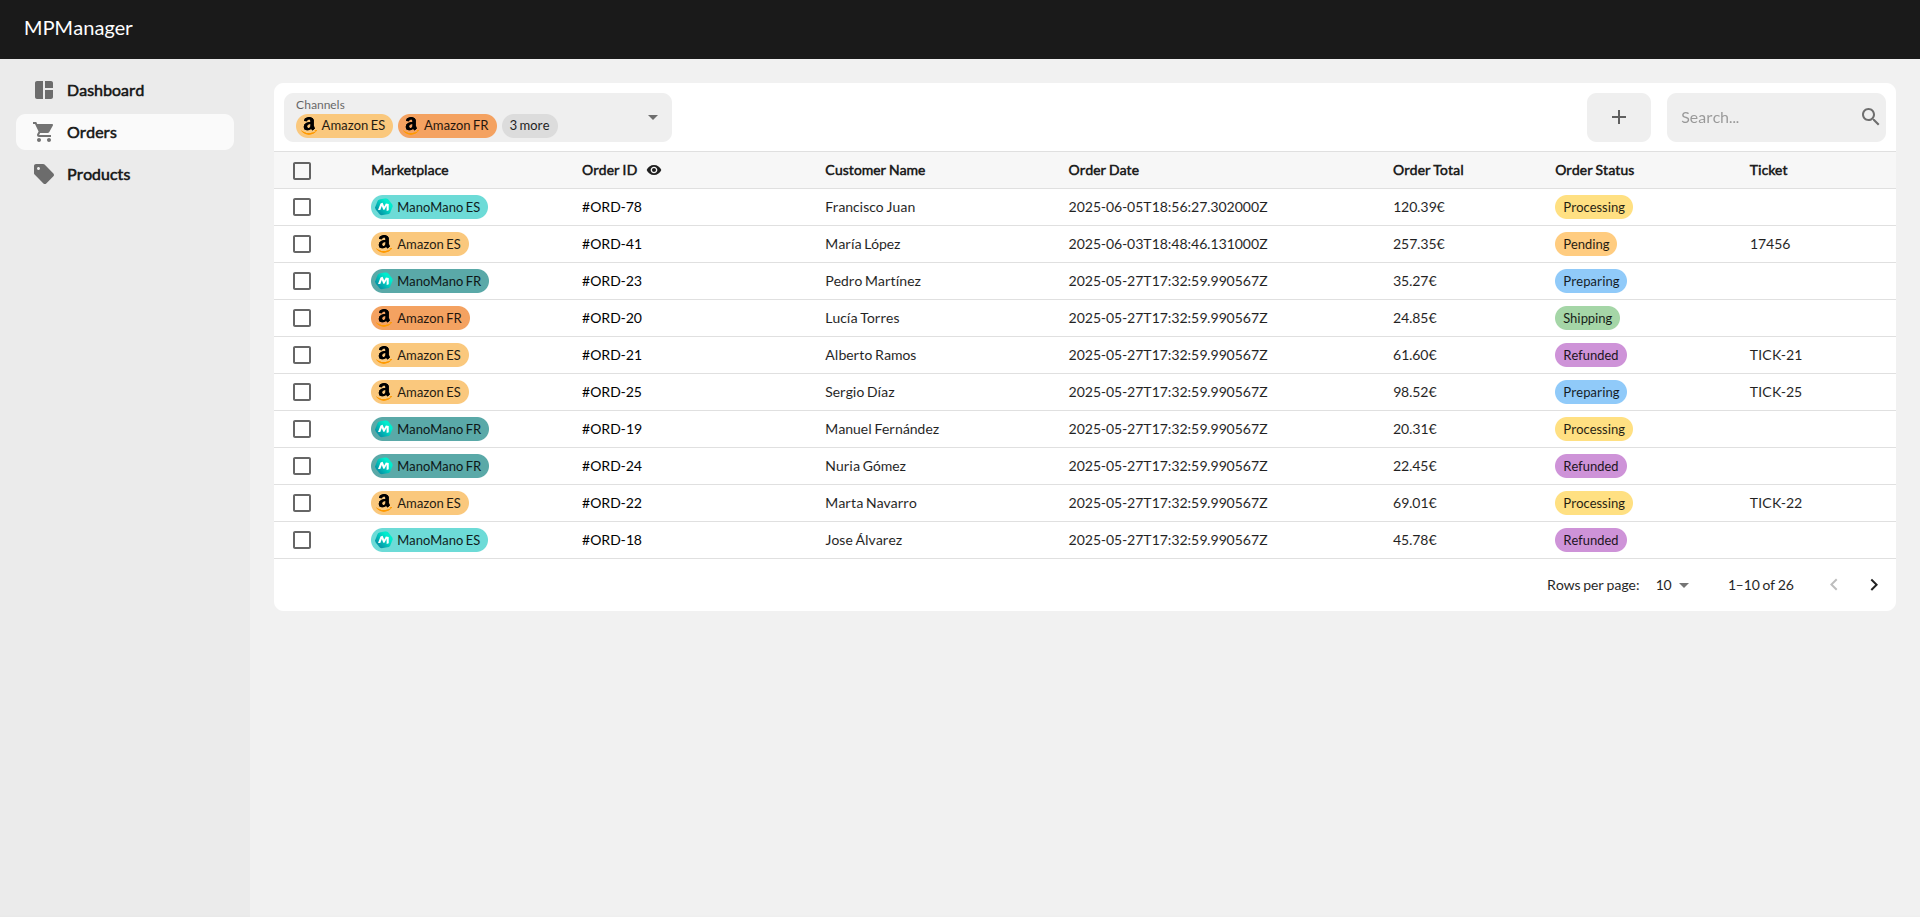
\includegraphics[width=0.8\textwidth]{figures/design_develop/screenshots/tabla_pedidos.png}
    \caption{Vista general de pedidos con algunos pedidos de ejemplo.}
    \label{fig:dev:ss:vista_general_pedidos}
\end{figure}

La primera de las vistas, la vista general de pedidos, es la que se muestra en la figura \ref{fig:dev:ss:vista_general_pedidos}. Esta vista está principalmente compuesta por una tabla que muestra los pedidos recibidos, mostrando el canal de venta del que provienen, el identificador del pedido, el nombre del cliente, la fecha de creación del pedido, el importe total y el estado del mismo. Adicionalmente, se ha añadido un campo de búsqueda que permite filtrar los pedidos por el identificador del pedido o el nombre del cliente; y un filtro por canal de venta que permite ver únicamente los pedidos de los canales seleccionados.

Sin embargo, se puede observar que la tabla no muestra todos los pedidos de la plataforma, sino que muestra únicamente los 10 últimos pedidos recibidos. Como un usuario puede tener cientos o miles de pedidos, es necesario implementar una paginación que permita navegar entre los distintos pedidos. Esta paginación implementada es la discutida en la sección \ref{dev:subsubsec:paginacion_endpoints}, y permite al usuario cambiar entre las distintas páginas de pedidos, seleccionar cuántos pedidos se quieren ver por página (10, 25, 50 o 100), buscar pedidos concretos y filtrar por canal de venta. De esta forma, para cada cambio de página, de búsqueda o de filtro, se realiza una petición al \textit{backend} para obtener los pedidos correspondientes a la página, búsqueda o filtro seleccionados.

\begin{figure}
    \centering
    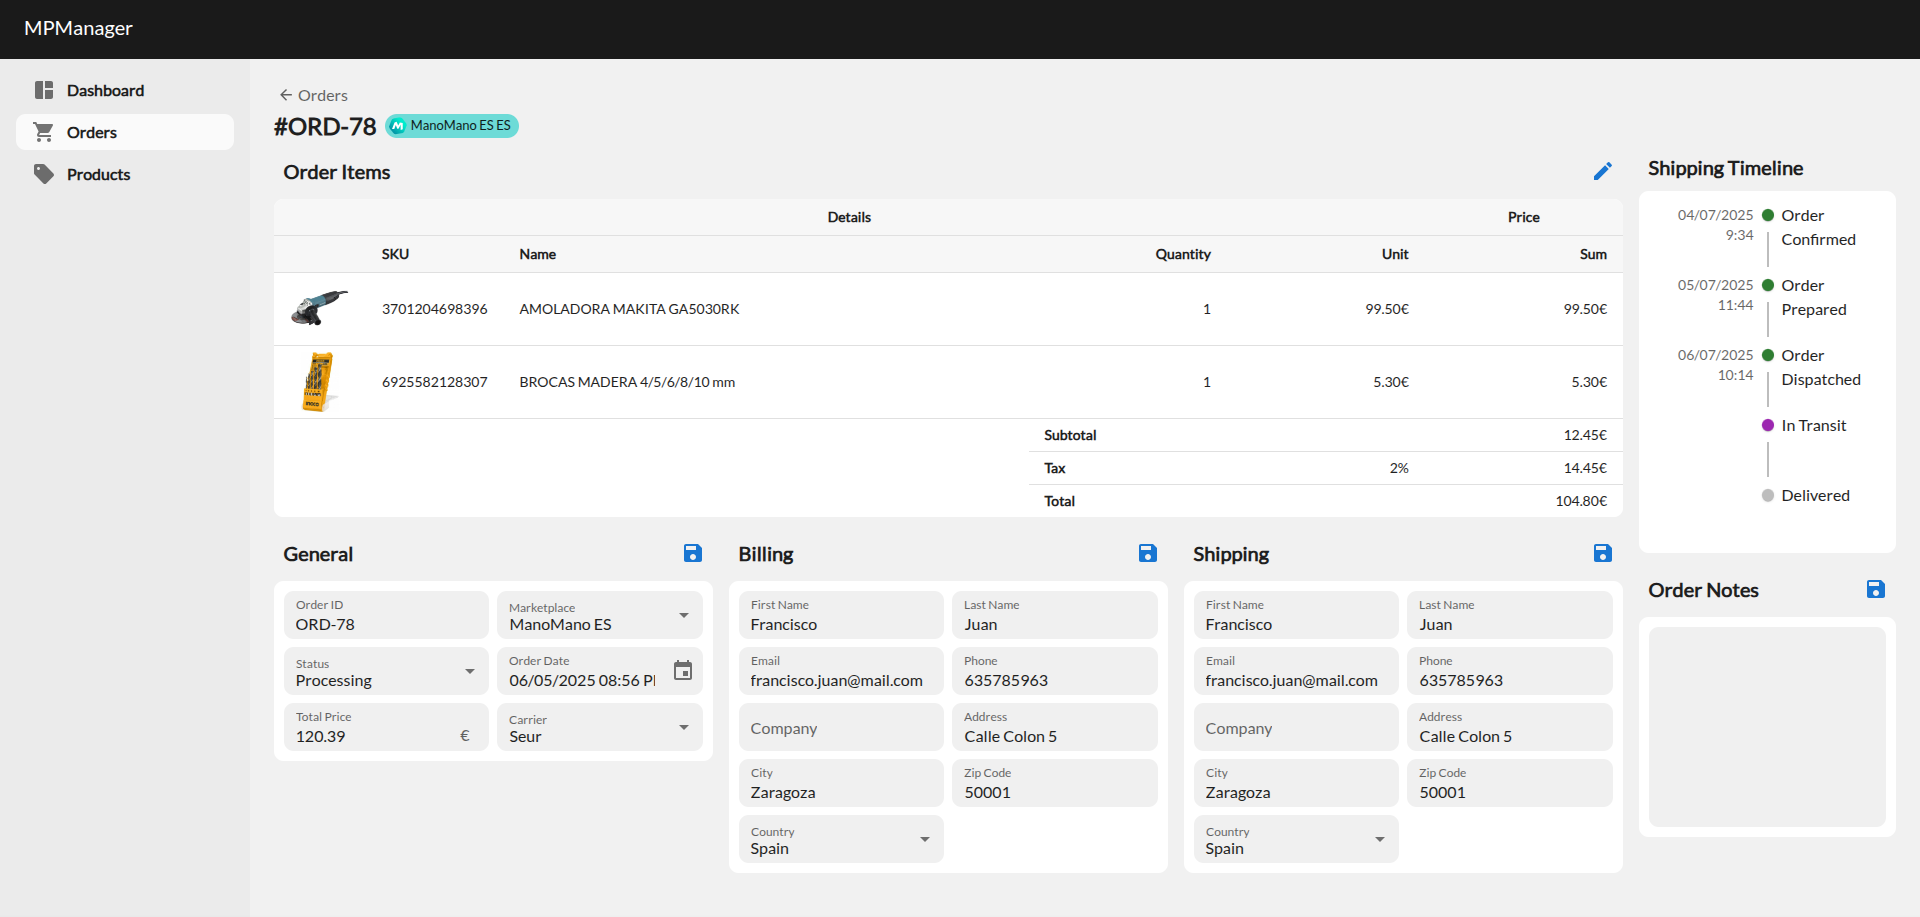
\includegraphics[width=0.8\textwidth]{figures/design_develop/screenshots/detalle_pedidos.png}
    \caption{Vista detallada de un pedido concreto.}
    \label{fig:dev:ss:vista_detallada_pedidos}
\end{figure}

Pulsando sobre un pedido concreto de la tabla, se accede a la vista detallada del pedido, que se muestra en la figura \ref{fig:dev:ss:vista_detallada_pedidos}. En esta vista se pueden ver todos los detalles del pedido, incluyendo los productos que lo componen, la información general del pedido y la información del cliente. Adicionalmente, se puede revisar cómo ha ido evolucionando el estado del pedido a lo largo del tiempo, ya que se muestra un historial de cambios de estado del pedido, y se pueden añadir notas para registrar información adicional relevante.

Existe la posibilidad también de editar el pedido, tanto los productos que lo componen como la información general y del cliente. Sin embargo, existe una restricción importante: solo se pueden editar los pedidos que hayan sido creados manualmente por el usuario. Los pedidos que provienen de los canales de venta no pueden ser editados, ya que su información es gestionada directamente por el canal de y no se permite modificarla manualmente. Esto asegura la integridad de los datos y evita posibles inconsistencias en la información. Tal como se muestra en la figura \ref{fig:dev:ss:campos_editables_pedido}, los únicos campos que se pueden editar en los pedidos provenientes de los canales de venta son el estado del pedido, el transportista, la dirección de envío y las notas del pedido. Estos campos son los que el usuario puede modificar para actualizar el estado del pedido o rectificar información para que el pedido pueda ser gestionado correctamente.

\begin{figure}[H]
    \centering
    \begin{subfigure}{\linewidth}
        \centering
        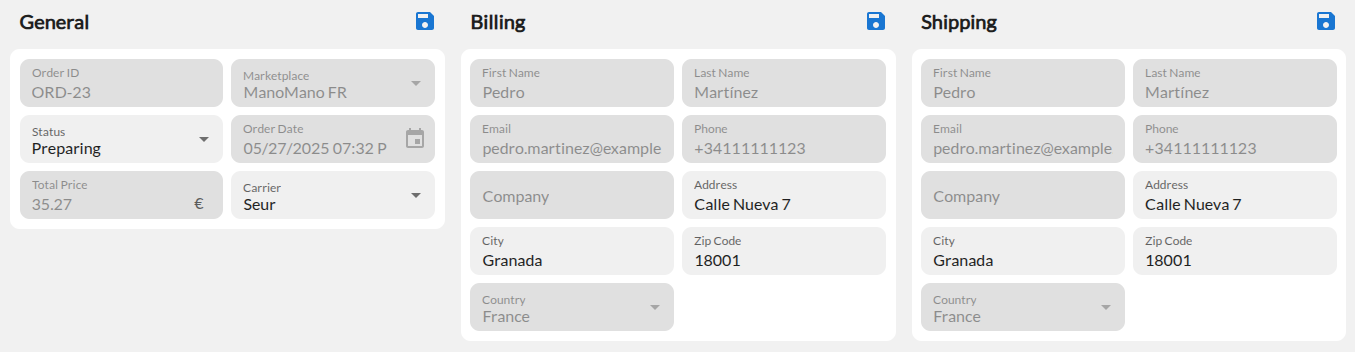
\includegraphics[width=0.8\linewidth]{figures/design_develop/screenshots/campos_bloqueados.png}
        \caption{Campos de un pedido creado automáticamente por el canal de venta.}
    \end{subfigure}
    \vspace{1em}
    \begin{subfigure}{\linewidth}
        \centering
        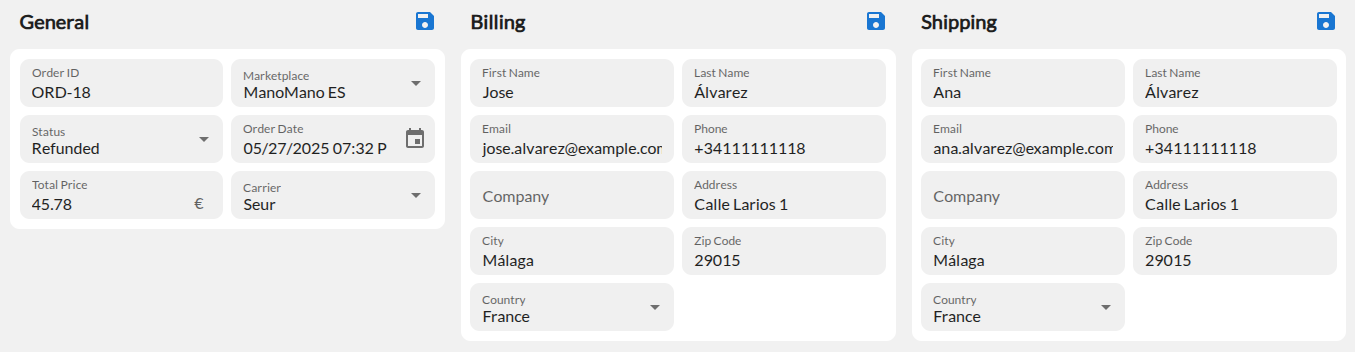
\includegraphics[width=0.8\linewidth]{figures/design_develop/screenshots/campos_no_bloqueados.png}
        \caption{Campos de un pedido creado manualmente por el usuario.}
    \end{subfigure}
    \caption{Campos editables de un pedido dependiendo de su origen.}
    \label{fig:dev:ss:campos_editables_pedido}
\end{figure}

En pedidos creados manualmente, se pueden añadir o quitar productos al pedido, así como editar los productos ya existentes. Para realizar estas acciones se debe pulsar el icono de edición que se encuentra en la parte superior derecha de la tabla de productos. Esto abrirá el modal que se muestra en la figura \ref{fig:dev:ss:modal_edicion_productos_pedido}, que permite añadir nuevos productos al pedido, así como editar la cantidad y el precio de los ya existentes, o hasta eliminarlos del pedido.

\begin{figure}
    \centering
    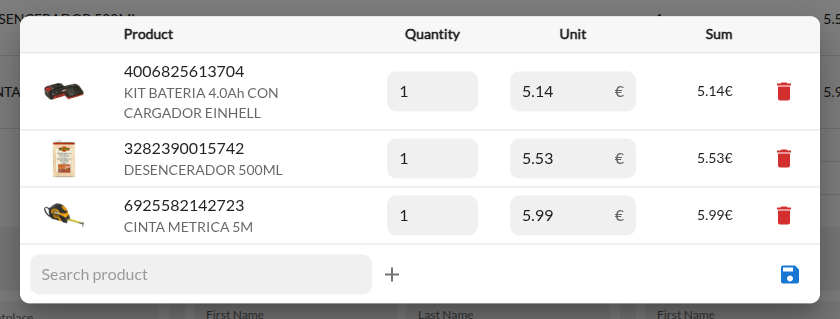
\includegraphics[width=0.7\textwidth]{figures/design_develop/screenshots/modal_edicion_productos_pedido.png}
    \caption{Modal de edición de productos de un pedido.}
    \label{fig:dev:ss:modal_edicion_productos_pedido}
\end{figure}

Este modal incluye características bastante complejas, como es la búqueda de productos dinámicamente. A medida que el usuario escribe en el campo de búsqueda el nombre o SKU del producto, se realiza una petición al \textit{backend} para obtener los productos que coinciden con la búsqueda. Solo los productos que se encuentran en el canal de venta del pedido se mostrarán en la lista de resultados, lo que asegura que solo se puedan añadir productos válidos al pedido. Además, para evitar que se hagan demanasiadas peticiones al \textit{backend}, se ha implementado un \textit{debounce} de 500 milisegundos, lo que significa que la búsqueda solo se realizará si el usuario deja de escribir durante ese tiempo. Esto reduce la carga en el servidor y mejora la experiencia del usuario al evitar peticiones innecesarias.

\begin{figure}[H]
    \centering
    \begin{subfigure}{0.45\linewidth}
        \centering
        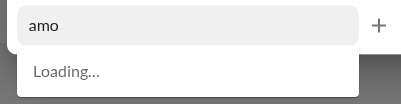
\includegraphics[width=\linewidth]{figures/design_develop/screenshots/busqueda_debounced_loading.png}
        \caption{Desplegable de búsqueda de productos con el \textit{debounce} mientras espera la respuesta del \textit{backend}.}
    \end{subfigure}
    \hfill
    \begin{subfigure}{0.45\linewidth}
        \centering
        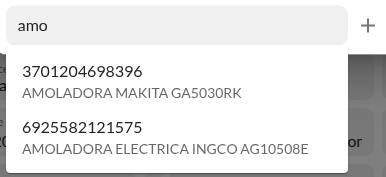
\includegraphics[width=\linewidth]{figures/design_develop/screenshots/busqueda_debounced.png}
        \caption{Desplegable de búsqueda de productos con los resultados obtenidos del \textit{backend}.}
    \end{subfigure}
    \caption{Proceso de búsqueda de productos con \textit{debounce}.}
    \label{fig:dev:ss:busqueda_debounced}
\end{figure}